\documentclass[11pt, a4paper]{article}
\usepackage[utf8]{inputenc}

\usepackage[margin=1in]{geometry} 
\usepackage{amsmath,amsthm,amssymb}
\usepackage[margin=1in]{geometry} 
\usepackage{amsmath,amsthm,amssymb}

\usepackage[slovene]{babel}
\usepackage{color}
\usepackage{graphicx}
\usepackage{amssymb}
\usepackage{amsmath}
\usepackage{mathtools}
\usepackage{commath}
\usepackage{ragged2e}
\usepackage[T1]{fontenc}
\usepackage[normalem]{ulem}
\usepackage{amsthm}
\usepackage{esvect}
\usepackage{float}
\usepackage{calrsfs}
\DeclareMathAlphabet{\pazocal}{OMS}{zplm}{m}{n}
\newcommand{\Ga}{\mathcal{G}}
\mathtoolsset{showonlyrefs} 

\newcommand\setItemnumber[1]{\setcounter{enumi}{\numexpr#1-1\relax}}


\newtheorem{theorem}{Trditev}[section]
\newtheorem{corollary}{Posledica}[section]
\newtheorem{lemma}[section]{Lema}
\theoremstyle{definition}
\newtheorem{definition}{Definicija}[section]
\theoremstyle{example}
\newtheorem{example}[section]{Primer}
\theoremstyle{izrek}
\newtheorem{izrek}[section]{Izrek}

\begin{document}
\begin{center}
\thispagestyle{empty}
\parskip=14pt%
\vspace*{3\parskip}%
\begin{Huge} Določitev osnovnega naboja po Milikanu \end{Huge}

By

Matic Tonin

ID No. (28181098)

Mentor 

(Rok Dolenec)

\rule{7cm}{0.4pt}

Pod okvirom:

FAKULTETE ZA FIZIKO IN MATEMATIKO, LJUBLJANA

4. 4. 2020

\end{center}
\pagebreak
\section{Naloga}
\begin{enumerate}
\item Izmeri hitrosti gibanja kapljic v gravitacijskem in elektricnem polju.
\item Iz meritev izracunaj velikosti kapljic in njihov naboj ter doloci osnovni naboj.
\end{enumerate}

Kljub temu, da meritve sam nisem izvajal, bom v poročilu navedel, kakšen bi moral biti postopek dela in kako smo dobili določene mertve. \\

\section{Postopek dela}
Najprej je bilo, kot je v navodilih napisano, treba pripraviti mikroskop, kondenzator in kamero. Nato smo oljne kapljice z gumjastim balonom razpršili po kondenzatorju. S spreminjanjem napetosti na kondenzatorju smo lahko opazili, da se kapljice premikajo v dve smeri, levo ali desno, odvisno od tega, v kateri fazi smo imeli naš preklopnik. Ko smo posneli enega izmed načinov, smo nato morali obdelati podatke na videu, kot nam narekujejo navodila. Več informacij podam pri samem načinu opazovanja. 

\section{Meritve}
\subsection{Merjenje radija na dva različna načina}
Najprej bom razložil, kako potekata oba načina, nato pa ju tudi predstavil na meritvah.
\begin{enumerate}
\item \underline{Merjenje radija v garavitacijskem polju}:  \\

Ko našo kapljico spustimo v gravitacijsko polje, ta začne prosto padati s silo $F=mg$. Maso kapljice lahko razpišemo z njenimi lastnostmi in sicer $m=V\rho_o=\frac{4\pi r^3}{3}\cdot \rho_o$. Torej dobimo, da je sila teže enaka:

$$F_g=\frac{4\pi r^3}{3}\cdot g \rho_o$$

Pri padanju kapljice skozi zrak pa delujeta še dve sili in sicer sila vzgona $F_{vzg}=\frac{4\pi r^3}{3}\cdot g \rho_z$ in Stokesova sila za kapljico, ali viskozna sila $F=6\pi r \eta v$. \\
Vemo, da sila viskoznosti in sila vzgona zavirata padanje, zato lahko napišemo enačbo, ki je bila zapisana že v uvodu. 

$$\frac{4\pi r^3}{3}\cdot g (\rho_o-\rho_z)=6\pi r \eta v$$

In z malo obračanja, lahko iz tega izrazimo radij kot: 
\begin{equation}
r^2=\frac{9\eta v}{2(\rho_o-\rho_z) g}
\label{Radij v gravitacijskem}
\end{equation}

Za drugi del vaje pa upoštevamo to, da ima kapljica olja v sebi večkratnik osnovnega naboja, kar pomeni da je naelektrena. Če tako kapljico postavimo v neko določeno električno polje, lahko povzročimo, da bo v njem lebdela in tako mirovala. Na njo bo še vedno delovala sila teže, sila vzgona, Stokesova sila pa bo tako enaka 0, pojavila pa se bo električna sila, ki bo nasprotovala gravitacijski.

\pagebreak 
Tako bo veljala zveza, da je: 

$$\frac{4\pi r^3}{3}\cdot g (\rho_o-\rho_z)=F_e$$

Za električno silo pa vemo, da je definirana kot $F_e=eE$ pri čemer je v naši kapljici $e=ne_0$. in ker vemo še, da je $E=\frac{U}{d}$, sledi:
\begin{equation}
\frac{4\pi r^3}{3}\cdot g (\rho_o-\rho_z)=ne_0\frac{U}{d}
\label{Naboj v gravitacijskem}
\end{equation}


\item \underline{Merjenje radija v električnem polju}\\
Za ta del pa lahko razmišljamo tudi drugače. Neko kapljico vzbujamo z našo napetostjo $U=dE$, kjer je d razdalja med ploščama tako, da kapljica še vedno pada, a le s počasnejšo hitrostjo. Zato nanjo še vedno deluje Stokesova sila in Newtonov zakon se tako glasi:

$$\frac{4 \pi}{3} r^{3}\left(\rho-\rho_{\mathrm{zr}}\right) g \pm|n| e_{0} E=\pm 6 \pi r \eta v_{\pm}$$

Če zapišemo obe enačbi, za negativno polje in pozitivno polje in ju nato seštejemo, lahko ven izrazimo radij. 
\begin{equation}
r^{2}=\frac{9 \eta\left(v_{+}-v_{-}\right)}{4 g\left(\rho-\rho_{\mathrm{zr}}\right)}
\label{Radij, električno polje}
\end{equation}


Če pa obe enačbi odštejemo med seboj, pa dobimo kar absolutno vresdnost večkratnika naboja. 

\begin{equation}
e_0=\frac{3\pi r \eta}{E}(v_++v_-)
\label{Naboj v električnem}
\end{equation}
\end{enumerate}

Sedaj smo definirali, kaj točno moramo početi s podatki in tako se lahko lotimo obdelave. 

\subsection{Meritve, ki jih poznamo že pred merjenjem}
Pred samo meritvijo imamo znanih kar nekaj podatkov, ki jih bomo navedli v spodnji tabeli. Nekaj podatkov je navedenih v uvodu, nekaj pa jih bomo poiskali po internetu.
\begin{table}[h]
	\centering
	\begin{tabular}{|c|c|}
		\hline
		Gostota olja, $\rho_o$ pri 23°C & 0.973 $\frac{g}{{cm}^3} \pm 0.001\frac{g}{{cm}^3}$ \\ [1ex]
		\hline
		Gostota zraka, $\rho_z$ pri 23°C & 1.194 $\frac{Kg}{{m}^3} \pm 0.001\frac{Kg}{{m}^3}$  \\[1ex]
		\hline
		Težni pospešek, g & 9.81 $\frac{m}{s}$ \\[1ex]
		\hline
		Viskoznost zraka, $\eta$ pri 23°C & 18.3 $\mu$Pas $\pm$ 0.01 $\mu$Pas \\[1ex]
		\hline
		Osnovni naboj, $e_0$ &  $1,602 \cdot 10^{-19}$ As \\[1ex]
		\hline
		Razmik med ploščama kondenzatorja, d & 5(1 $\pm$ 0.02) mm \\[1ex]
		\hline
	\end{tabular}
	\caption{Začetni podatki za naše meritve}		\label{osnove}
\end{table}

\pagebreak
\subsection{Merjenje v gravitacijskem pospešku}
\subsubsection{Radij}
Kot podatke smo merili hitrosti naših kapljic in preko zveze (\ref{Radij v gravitacijskem}), ki je zapisana v poglavju 3.1.1. lahko dobimo tudi radij.
Podatkov ne bom navajal v svojem poročilu zaradi njihove obsežnosti, navedel pa bom zgolj graf hitrosti v odvisnosti od radijev v $\mu m$ in v $\frac{\mu m}{s}$. 
\begin{figure}[H]
	\centering
    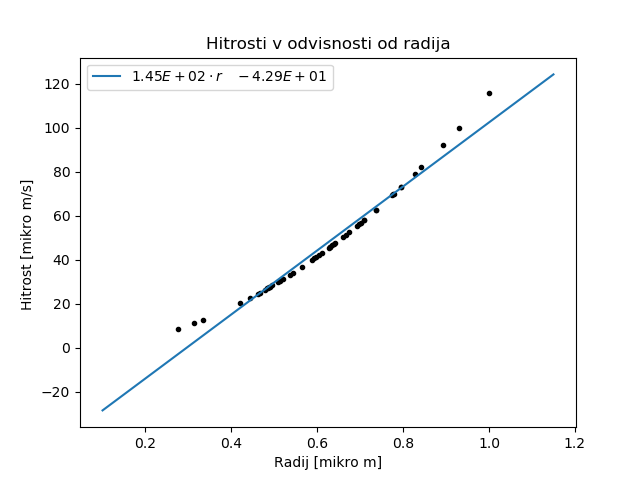
\includegraphics[width=12cm]{Hitrosti.png}
    \caption{Prikaz hitrosti v odvisnosti od radija na grafu}
\end{figure}

Izračunane podatke pa lahko navedemo v tabeli: 
\begin{table}[h]
	\centering
	\begin{tabular}{|c|c|}
	\hline
	\hline
	Koeficient premice, K & $1.45 \cdot 10^{2} \cdot r $\\
	\hline
	Povprečje radijev, $\overline{r}$ & $0.62 \mu m$ \\
	\hline
	\end{tabular}
	\caption{Podatki o hitrostih in radijih pri meritvi z gravitacijo}		
\end{table}

\subsubsection{Naboj}
Za izračuna naboja pa si pomagamo z formulo (\ref{Naboj v gravitacijskem}), pri čemer bomo morali upoštevat radije iz prejšnje meritve. 
V dodatnih navodilih za obdelavo vidimo, da nam koristijo zgolj kapljice, katerih n<6, zato sestavimo program, ki nam izračuna vrednost $ne_0$ ter nato izpiše, koliko kapljic ima večji naboj. Ugotovili smo, da je to zgolj ena sama kaplijica in sicer z nabojem: $1.0008442322145073\cdot 10^{-18} As$.

Po izračunu vseh kapljic, lahko izračunamo, kolikšno je povprečje naboja iz vseh in sicer dobimo, da je:

$$\overline{e_o}= 1.59\cdot 10^{-19} $$

Kako sem to točno naredil?
Za vsako kapljico posebej je program preveril, koliko je razmerje med $ne/e_0$ in ga nato ocenil na naravno število. Nato pa sem lahko, ko sem vedel, koliko je faktor n za vsako kapljico, lahko izračunal vrednosti $e_0$ za vsako kapljico posebej in naredil povprečje. 

\pagebreak

Sedaj pa potrebujemo izmeriti zgolj še histogram razporeditve kapljic glede na naboj. Za to bomo ponovno uporabili program, ki nam bo najprej indeksiral kapljice glede na to, koliko kapljic je imelo določen n kratnik naboja po intervalih in nam zrisal histogram, ki ga želimo. Tako dobimo:

\begin{figure}[H]
	\centering
    \includegraphics[width=12cm]{Gravitacija,histogram.png}
    \caption{Histogram porazdelitve nabojev v odvisnosti od naboja}
\end{figure}
Če pa razporedimo naboje kapljic po velikosti in jih nato indeksiramo vsako po sebej ter opazujemo elekrične skoke med njimi, pa dobimo histogram:
\begin{figure}[H]
	\centering
    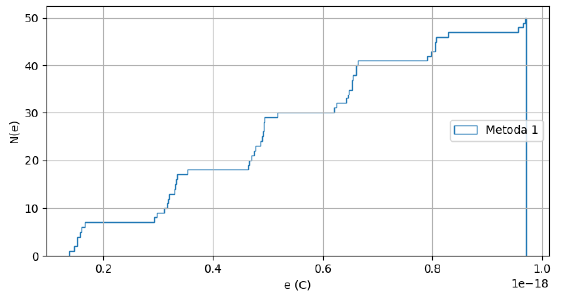
\includegraphics[width=12cm]{Pravilen histogram,GM.png}
    \caption{Histogram porazdelitve nabojev v odvisnosti od naboja}
\end{figure}

Tudi na histogramu se vidi, da je prva točka, kjer se naboj začne ohranjati in to je približno pri 1.6 $10^{-19}$ As.

\pagebreak
\subsection{Meritev v električnem polju}
\subsubsection{Radij}
Kot podatke smo merili hitrosti v eni in drugi smeri in preko zveze (\ref{Radij, eletrično polje}) lahko dobimo tudi radij. Podatkov ne bom navajal v svojem poročilu zaradi njihove obsežnosti, navedel pa bom zgolj graf razlike hitrosti v odvisnosti od radijev. 
\begin{figure}[H]
	\centering
    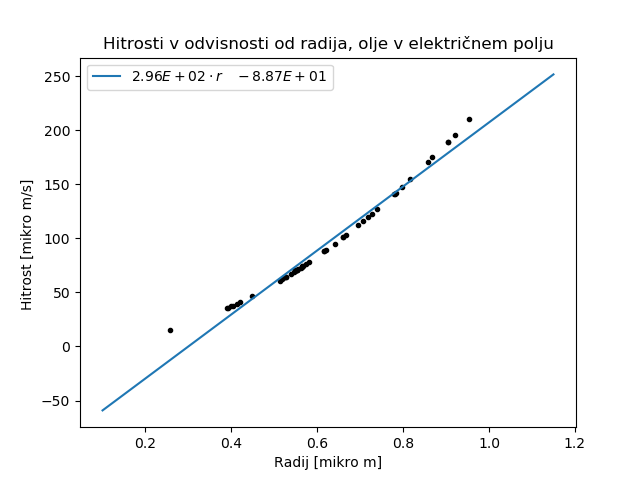
\includegraphics[width=12cm]{Elektrika,Radij-hitrost.png}
    \caption{Graf odvisnosti razlike hitrosti od radija kapljice}
\end{figure}
Izračunane podatke pa lahko navedemo v tabeli: 
\begin{table}[h]
	\centering
	\begin{tabular}{|c|c|}
	\hline
	\hline
	Koeficient premice, K & $2.96 \cdot 10^{2} \cdot r $\\
	\hline
	Povprečje radijev, $\overline{r}$ & $0.619 \mu m$ \\
	\hline
	\end{tabular}
	\caption{Podatki o hitrostih in radijih pri meritvi z električnim poljem}
\end{table}

\subsubsection{Naboj}
Za izračuna naboja pa si pomagamo z formulo (\ref{Naboj v električnem}), pri čemer bomo morali upoštevat radije iz prejšnje meritve. 

Po izračunu vseh kapljic, lahko izračunamo, kolikšno je povprečje naboja iz vseh in sicer dobimo, da je:

$$\overline{e_o}= 1.61\cdot 10^{-19} $$

Kako sem to točno naredil?
Za vsako kapljico posebej je program preveril, koliko je razmerje med $ne/e_0$ in ga nato ocenil na naravno število. Nato pa sem lahko, ko sem vedel, koliko je faktor n za vsako kapljico, lahko izračunal vrednosti $e_0$ za vsako kapljico posebej in naredil povprečje.


Sedaj pa potrebujemo izmeriti zgolj še histogram razporeditve kapljic glede na naboj. Za to bomo ponovno uporabili program, ki nam bo najprej indeksiral kapljice glede na to, koliko kapljic je imelo določen n kratnik naboja po intervalih in nam zrisal histogram, ki ga želimo. Tako dobimo:
\begin{figure}[H]
	\centering
    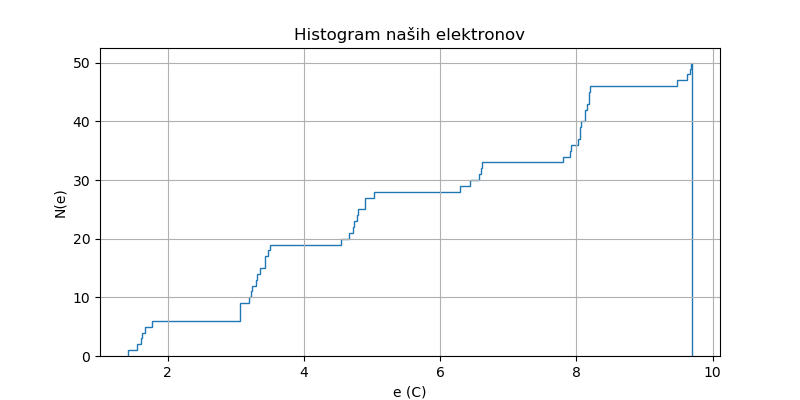
\includegraphics[width=12cm]{Pravilen histogram,E.png}
    \caption{Histogram porazdelitve nabojev v odvisnosti od naboja}
\end{figure}

Tudi tu vidimo,  da pride do ustalitve nabojev okoli 1.6 $10^{-19}$ As.

\section{Zaključek}
Na podlagi znanja, da se lahko naboj prenaša samo v večkratnikih in s po-
služevanjem asimetrije med naelektrenih delcev proti ali z električnim poljem,
sem lahko uspešno dokaj natančno določil osnovni naboj z Millikanovim po-
skusom. Za boljšo natančnost bi lahko meril večkrat, a je tudi ta rezultat
zadovoljiv. Predvsem zanimivo je, da lahko na podlagi preskokov ocenimo,
kje se večkratnost naboja spremeni. Z majhnim količinom kaplic tega ne bi
mogli narediti.
\end{document}